\onecolumn
\section*{\LARGE Supplementary Material}
\label{sec:appendix}

% \section{Full Pipeline Pseudo-code}
% Algorithm~\ref{alg:dlm} in the main text presents a phase-level overview. Below, we give the full pseudo-code in Algorithm~\ref{alg:pipeline-full}.
% Each source unit $u \in \mathcal{U}$ and each agent reasoning trace $\Rsto$ contributes an entry to this shared context $\sctx$ through a hierarchical transformation. Specifically, a first-stage summarizer $\phi_1$ produces a reference-grounded summary $S$, and a second-stage summarizer $\phi_2$ further compresses $S$ into a highly compact gist $G$. Only $G$ is admitted to $\sctx$, while $S$ and the raw content are retained in addressable stores $\mathcal{L}$ and $\mathcal{R}$ to support later selective unfolding. Verification is enforced at the moment $S$ and $G$ are produced, ensuring that only verified gists enter $\sctx$. 

% The code will be released upon acceptance.

% \begin{algorithm}[!h]
% \caption{\toolName{} pipeline. \plug{Highlighted} components are pluggable (see \S\ref{sec:method}, second paragraph).}
% \label{alg:pipeline-full}
% \begin{algorithmic}[1]
% \Require Question $Q$; optional source units $\mathcal{U}$ (default $\emptyset$)
% \Ensure Final answer $Y$
% \Statex \textit{$\sctx$---shared context; $\mathcal{L},\mathcal{R}$---per-entry stores for $S$ and raw; $\mathcal{T}$---task queue; $\ell$---labels for $u, t$.}
% \State $C \leftarrow [\,]$;\ \ $\mathcal{L}, \mathcal{R} \leftarrow \emptyset$

% \If{$\mathcal{U} \neq \emptyset$}
%     \ForAll{$u \in \mathcal{U}$ \textbf{in parallel}}\Comment{seed: summarize, verify, and admit each source}
%         \State $S \leftarrow$ \plug{$\phi_1$}$(u;\, Q, C)$;\ \ $G \leftarrow$ \plug{$\phi_2$}$(S;\, Q, C)$ with \plug{\textsc{Verify-U}}$(G, S, u)$
%         \State $\mathcal{R}[\ell] \leftarrow u$;\ \ $\Lsto[\ell] \leftarrow S$;\ \ append $(\ell, G)$ to $\sctx$
%     \EndFor
% \EndIf

% % \Statex \textbf{Plan, run agents, verify outputs, replan as needed.}
% \State $\mathcal{T} \leftarrow$ \plug{\textsc{Plan}}$(Q, C)$
% \While{$\mathcal{T} \neq \emptyset$}
%     \ForAll{ready task $t \in \mathcal{T}$ \textbf{in parallel}}\Comment{$N$ agents pop concurrently from $\mathcal{T}$}
%         \State $r \leftarrow$ \plug{\textsc{RunAgent}}$(t, C, \mathcal{L}, \mathcal{R})$ \Comment{agent reads $\sctx$; unfolds $\mathcal{L}, \mathcal{R}$ on demand}
%         \State $S \leftarrow$ \plug{$\phi_1$}$(r;\, Q, C)$;\ \ $G \leftarrow$ \plug{$\phi_2$}$(S;\, Q, C)$
%         \State $(ok,\, \rho) \leftarrow$ \plug{\textsc{Verify-T}}$(G, S, r)$ \Comment{$\rho$: rejection reason when $\neg ok$}
%         \If{$ok$}
%             \State $\mathcal{R}[\ell] \leftarrow r$;\ \ $\Lsto[\ell] \leftarrow S$;\ \ append $(\ell, G)$ to $\sctx$
%         \Else
%             \State $\mathcal{T} \leftarrow \mathcal{T} \cup \{(t,\, \rho)\}$ \Comment{re-queue $\tque$ with rejection reason $\rho$}
%         \EndIf
%     \EndFor
%     \If{$\mathcal{T} = \emptyset$}
%         \State $\mathcal{T} \leftarrow$ \plug{\textsc{Replan}}$(Q, C)$
%         \Comment{can return empty}
%     \EndIf
% \EndWhile
% \State \Return $Y \leftarrow$ \plug{\textsc{Finalize}}$(Q, C, \mathcal{L}, \mathcal{R})$ \Comment{finalizer may unfold $\mathcal{L}, \mathcal{R}$ on demand}
% \end{algorithmic}
% \end{algorithm}


% % \section{Detailed Comparison with RLM}\label{sec:comp_rlm}
% % Here, we highlight four key differences between \toolName{} and RLM~\citep{zhang2025recursive}.

% % \paragraph{(1) Intra-trajectory refinement vs.\ shared-state construction.}
% % RLM performs {intra-trajectory refinement}: a single model recursively spawns sub-calls, consumes their outputs, and continues reasoning within one overall control flow. These intermediate results can improve the current trajectory, but they do not constitute a persistent shared representation that multiple agents can independently read, update, and build upon. \toolName{}, in contrast, is organized around {shared-state construction}: each source unit and completed subtask contributes a verified gist to a shared context that is visible to all agents by default. The objective is therefore not only to improve a single reasoning trajectory, but to construct a stable global view of the evidence accumulated so far.

% % \paragraph{(2) Raw-token selection vs.\ semantic progressive selection.}
% % RLM treats the long prompt as an external environment and recursively selects raw snippets to inspect, so planning is based on a limited view of the context and the model must repeatedly decide which regions to open next. \toolName{} instead plans over a verified shared context: agents first see high-level semantic gists \(G_i\) of the corpus, then progressively unfold relevant sources into reference-grounded summaries \(S_i\), and finally access raw evidence only when needed. This turns selection from a repeated raw-token search problem into a cumulative semantic refinement process, where global structure guides fine-grained retrieval.

% % \paragraph{(3) Unverified intermediate results vs.\ verified shared communication.}
% % RLM does not explicitly treat summary formation as a reliability bottleneck: intermediate results may guide later recursive calls, but there is no admission-time mechanism that enforces faithfulness before those results are reused. This is less problematic in a single-agent trajectory, where the broader trace remains available for later revision. In a multi-agent setting, however, summarized communication creates a sharper failure mode: once a distorted intermediate result enters the shared context, it can propagate as a false premise for all downstream agents. \toolName{} addresses this by verifying summaries at the moment they are written, while the underlying trace or source evidence is still available. Thus, the shared context is not only compact, but also more reliable, inspectable, and suitable for reuse by other agents.

% % \paragraph{(4) Centralized orchestration vs.\ decentralized coordination.}
% % The communication topology also differs fundamentally. RLM is {centralized}: a root reasoner coordinates recursive calls and aggregates their outputs through an explicit control structure. \toolName{} is {decentralized}: agents coordinate implicitly by reading from and writing to the same verified shared context. This removes the need for a single controller to mediate every information flow, and allows coordination to scale through a curated common substrate rather than through repeated centralized aggregation. In this sense, \toolName{} turns intermediate reasoning products into a shared system state, rather than treating them only as temporary outputs inside one recursive trace.

\begin{figure}[!h]
    \centering
    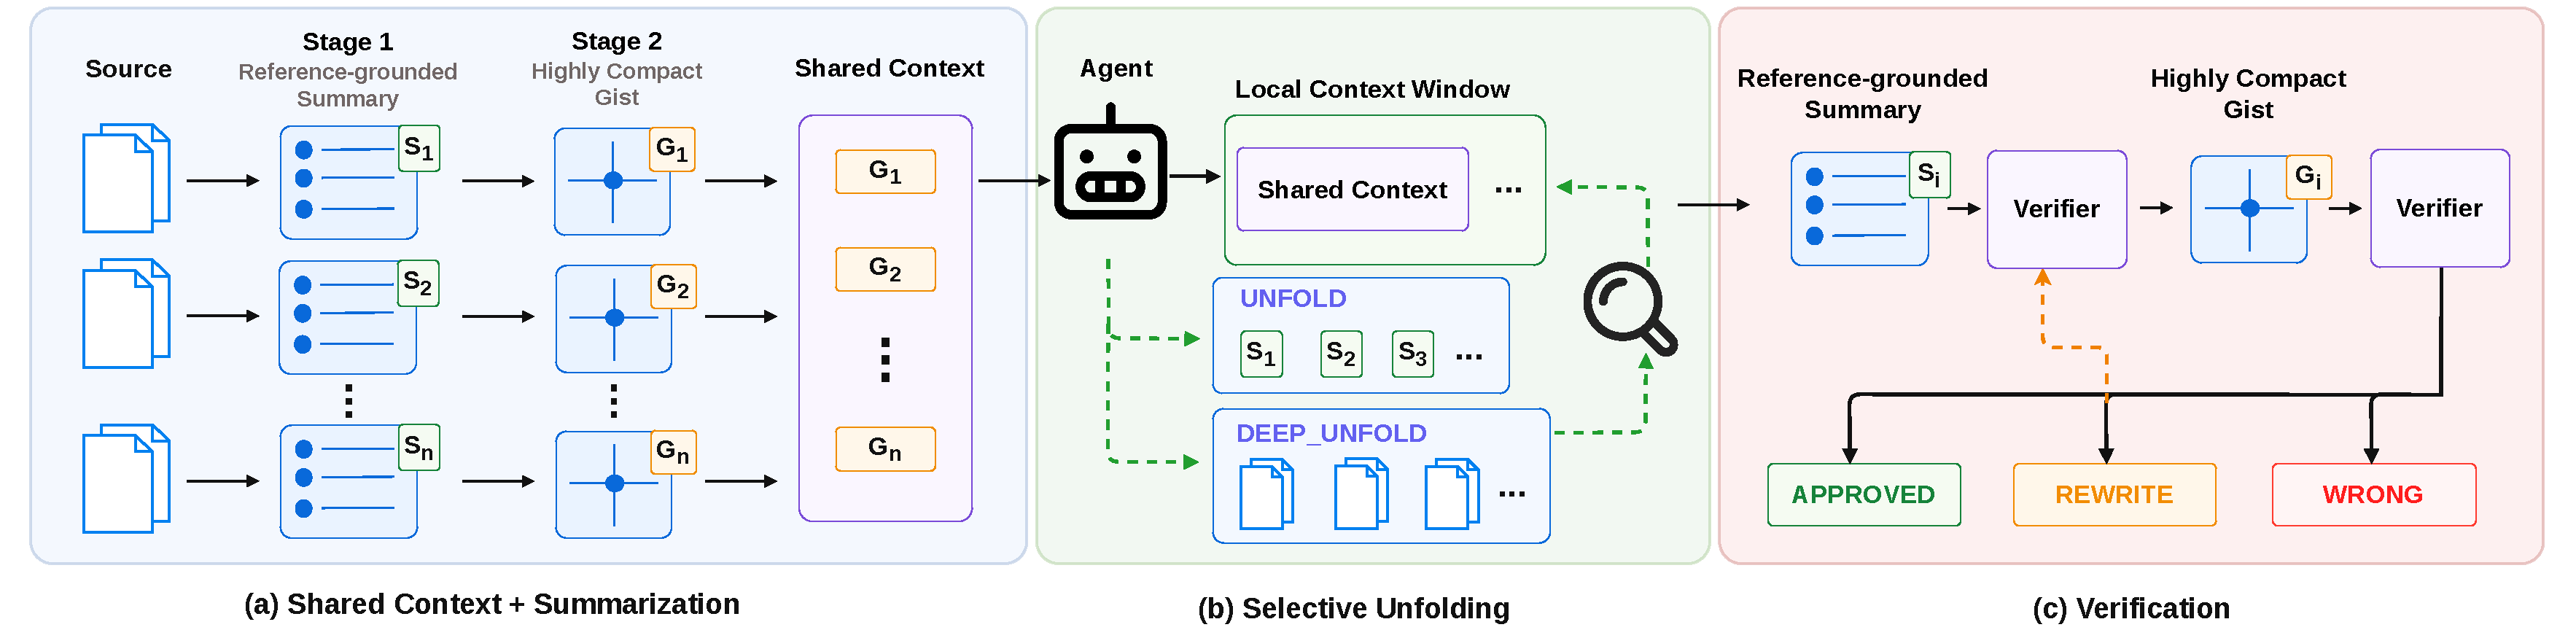
\includegraphics[width=1\linewidth]{modular.pdf}
    \caption{(a) Long source units are compressed into reference-grounded summaries $S_i$ and then compact gists $G_i$ stored in the shared context. (b) Agents read gists by default, selectively unfold them to summaries or raw evidence when needed, and (c) admit entries only after verification.}
    \label{fig:shared_context}
\end{figure}

\section{Method Details}

\subsection{Hierarchical Summarization}
\label{sec:summarization}
For long source units $r_i$ with label $\ell_i$, \toolName{} uses a three-level representation, $r_i \rightarrow S_i \rightarrow G_i$. The shared context $\sctx$ stores only compact gist entries $(\ell_i, G_i)$, giving every agent a lightweight global view of the corpus. The detailed backing content is stored outside $\sctx$: $\Lsto[\ell_i]$ contains the reference-grounded summary $S_i$, and $\Rsto[\ell_i]$ contains the corresponding raw source unit.

This hierarchy avoids relying on a lossy gist to directly select raw evidence while also avoiding broad raw-context unfolding. Agents first reason over gists, then unfold to $S_i$ or raw evidence only when finer-grained support is needed. For reasoning trajectories, \toolName{} usually admits a direct gist $G_i$, since later agents typically need the distilled finding, failure, feedback, or constraint rather than the full trace; the original trajectory remains available in $\Rsto[\ell_i]$ when needed.

We now describe the hierarchical summarization path for long source units.

\paragraph{Stage 1: $S_i$ (ref-grounded evidence map).}
Given a source unit $u_i$, the first-stage summarizer $\phi_1$ produces an evidence map consisting of a set of short bullets, each expressing a single atomic claim. Every bullet includes a {ref-tag} that identifies its supporting span in the raw text:
\begin{equation}
    \texttt{[ref: } h \;\ldots\; t\,\texttt{]},
\end{equation}
where $h$ and $t$ denote the first and last $N \geq 5$ words of the supporting span, respectively, copied verbatim. Formally,
\begin{equation}
    S_i = \phi_1(u_i;\, Q) = \{(b_{i,k},\, \reftag_{i,k})\}_{k=1}^{m_i}, \quad \reftag_{i,k} = (h_{i,k}, t_{i,k}),
\end{equation}
where $b_{i,k}$ is the $k$-th bullet and $\reftag_{i,k}$ is its ref-tag. $\phi_1$ is conditioned on the question $Q$ so that question-relevant content is extracted at higher fidelity. Full coverage of the source unit is required, as any portion may contain the critical evidence needed to answer the question. The resulting $S_i$ is stored in $\Lsto[\ell_i]$, with each bullet addressable by its local index $k$.

% The ref-tag mechanism makes Stage 1 verifiable: each concrete claim is explicitly grounded in a source span, enabling efficient validation without re-reading the full raw content.

\paragraph{Stage 2: $G_i$ (compact shared-context entry).}
A second-stage summarizer $\phi_2$ compresses $S_i$ into a short, highly compact gist:
\begin{equation}
    G_i = \phi_2(S_i;\, Q).
\end{equation}
This gist captures the relevance of $u_i$ to the query at a density that allows downstream agents to decide, at a glance, whether further inspection is needed. Only $G_i$ is admitted to $\sctx$, while $S_i$ and the raw content remain in $\mathcal{L}$ and $\mathcal{R}$ and are accessed only through selective unfolding (\S\ref{sec:unfold}).

% \yuzhen{Add the LLM-assist split boundaries strategy, and the coverage guarantee. Also introduce using cheap model for large corpus compression, with reference}

% \begin{figure}[!t]
%     \centering
%     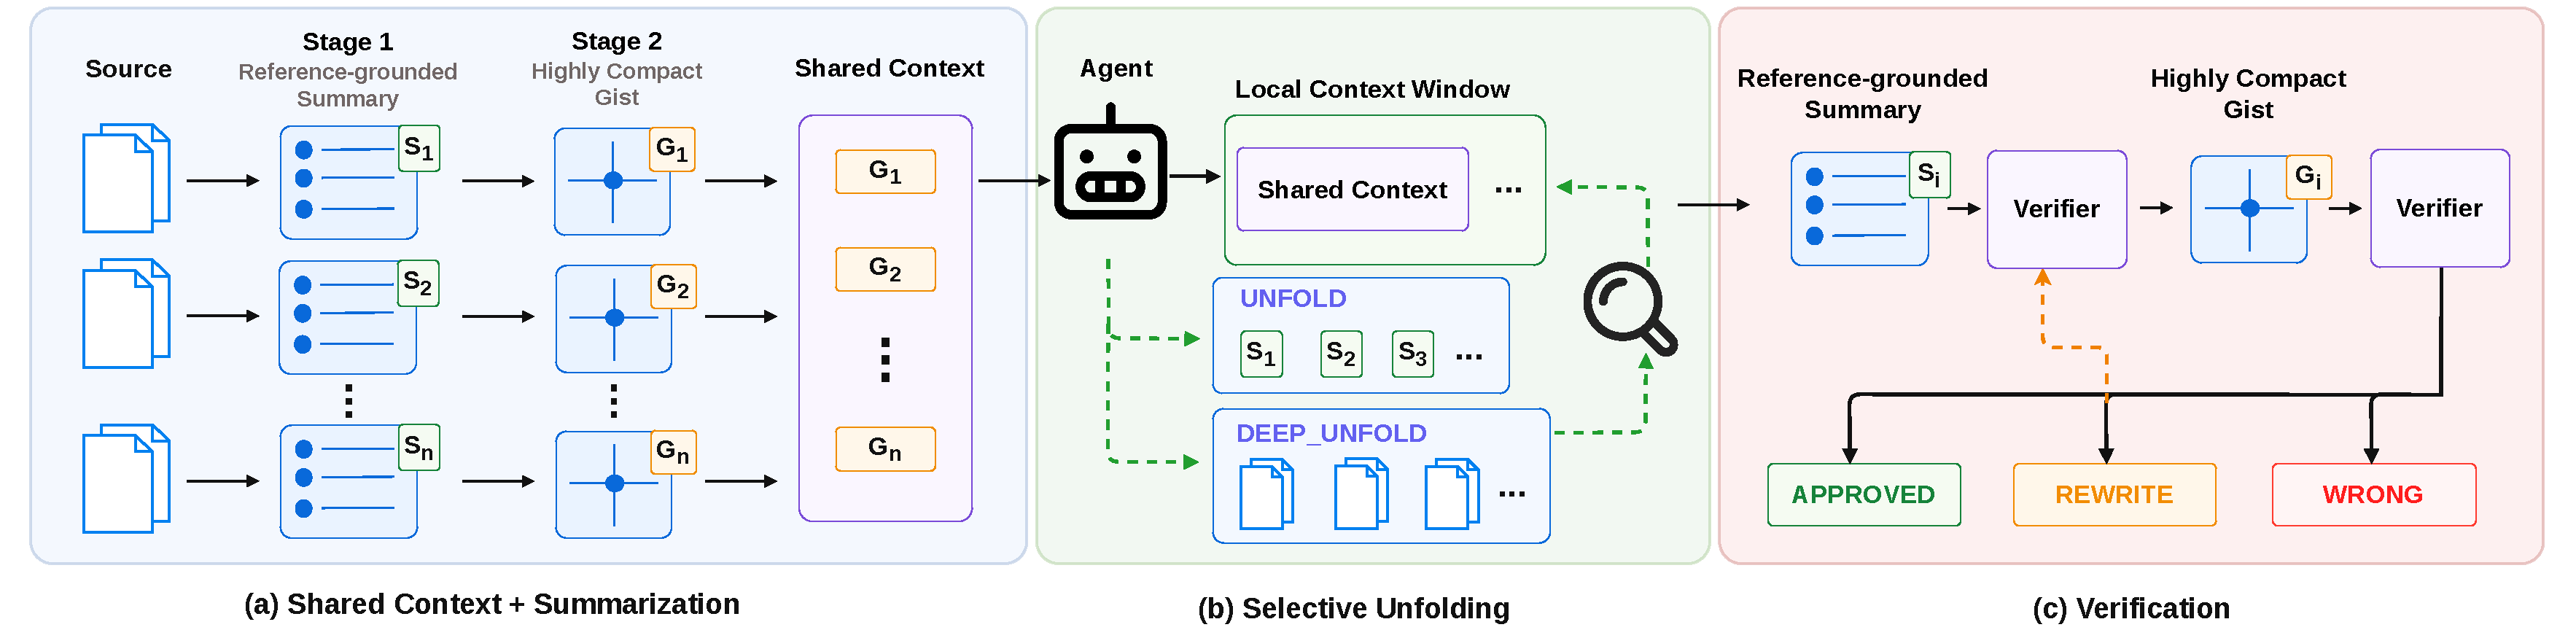
\includegraphics[width=1.0\linewidth]{modular.pdf}
%     \caption{Three core modules of \toolName{} (illustrated using the source-unit case). {(a) Shared Context + Summarization:} each source is summarized hierarchically into a reference-grounded summary $S_i$ and a compact gist $G_i$; only $G_i$ is admitted to the shared context. {(b) Selective Unfolding:} agents reason over the shared context by default and progressively unfold relevant entries to $S_i$ (\texttt{UNFOLD}) or to raw sources (\texttt{DEEP\_UNFOLD}) on demand. {(c) Verification:} both $S_i$ and $G_i$ are validated against their underlying evidence and routed to one of three outcomes: \textsc{Approved}, \textsc{Rewrite}, or \textsc{Wrong}.}
%     \label{fig:modular}
% \end{figure}

\subsection{Selective Unfolding}
\label{sec:unfold}
Agents reason over the shared context $\sctx$ by default, using the compact $G_i$ entries. When additional detail is required, they invoke {selective unfolding}, a coarse-to-fine, opt-in mechanism for retrieving more detailed information on demand. We implement unfolding in two stages: first, from $G_i$ to the reference-grounded summary $S_i$, and then, if necessary, from $S_i$ to the raw source content.

% \yuzhen{Hierarchical, coarse to fine search, Make sure both broad and deep requirement, Include neighborhood and also consider the coverage. Hybrid gist and summary search combination}

\paragraph{Stage 1: $G \rightarrow S$ (\texttt{UNFOLD}).}
At any reasoning step, the agent may request a small set of labels via an \texttt{UNFOLD: $\ell_1, \ell_2, \ldots$} directive. The orchestrator retrieves the corresponding $S_i$ summaries $\Lsto[\ell]$ and inlines their bullet-level evidence maps into the agent’s prompt for that call. This enables the agent to reason over grounded evidence rather than compressed gists.

\paragraph{Stage 2: $S \rightarrow \text{raw}$ (\texttt{DEEP\_UNFOLD}).}
After reasoning over the $S_i$ summaries, the agent may determine that finer-grained detail is required---for example, to resolve subtle qualifiers or verify exact wording. It can then emit a \texttt{DEEP\_UNFOLD: $\ell_1, \ldots$} directive specifying the labels whose raw content is needed. The orchestrator issues a follow-up call that combines the original task, the shared context $\sctx$, the previously unfolded summaries $S_i$, and the newly requested raw content from $\mathcal{R}$.

Unfolding proceeds in a coarse-to-fine, on-demand manner and may span multiple rounds up to a fixed limit, with each round allowing the agent to request additional $S_i$ or raw content as needed. Additionally, raw retrieval is also neighborhood-aware: requesting sub-chunk $n$ returns $n{\pm}1$ as well, which helps absorb off-by-one citation errors. Importantly, unfolded content is local to the requesting call and is not written back to the shared context $\sctx$, so subsequent agents still observe only the gist layer. This design prevents detailed intermediate content from polluting the shared context while preserving access to fine-grained evidence when necessary. As a result, the cost of detailed inspection scales with the amount of information actually required, rather than the total volume of available context.

\subsection{Admission-Time Verification}
\label{sec:verification}
Verification follows the compression path. For a reasoning trajectory, \toolName{} checks whether the gist $G_i$ faithfully preserves the relevant finding, failure, feedback, or constraint from the original result $r_i$. For a long source unit, \toolName{} verifies both levels of the hierarchy, first grounding the Stage-1 summary $S_i$ in the raw source and then checking the Stage-2 gist $G_i$ against $S_i$.

Specifically, each Stage-1 bullet $b$ with a reference $(h,t)$ is accepted only if the head $h$ and tail $\tque$ both appear, in order and verbatim, in the underlying source unit $u$. Bullets that fail this condition are routed to a targeted rewrite step, which either supplies a valid reference or drops the claim.

After this gate, an {iterative coverage loop} identifies large uncovered regions, defined as contiguous spans not referenced by any admitted bullet, and requests additional bullets for each gap. Newly generated bullets must pass the same reference and semantic-support checks before being added to $S_i$. The loop terminates when no large gaps remain or a fixed iteration limit is reached.

The Stage-2 gist $G_i$ is then produced from the verified $S_i$. Because $S_i$ contains only grounded claims, $G_i$ inherits this grounding at a coarse level. To guard against abstraction errors, $G_i$ undergoes a lightweight verification step using a cheaper LLM, such as DeepSeek-V4-Flash, which checks for hallucinations, semantic drift, and missing critical qualifiers relative to $S_i$. Only gists that pass this check are admitted to $\sctx$; otherwise, the update is rejected, regenerated, or returned to the task queue $\mathcal{T}$ with a rejection reason, up to a fixed retry limit.

% The verifier returns one of three outcomes: \textsc{Approved}, \textsc{Rewrite}, or \textsc{Wrong}. In the first two cases, a corrected and verified summary is produced and admitted as $G$. In the \textsc{Wrong} case, the task is returned to the task queue $\mathcal{T}$ with rejection reason, up to a fixed retry limit. As a result, every entry admitted to the shared context has passed an explicit grounding check and retains a traceable link to its supporting evidence. Because each $G$ entry preserves an addressable path through $S$ to its source ($u$ or $\Rsto$), any agent can later re-audit a suspect entry by traversing $\mathcal{L}$ and $\mathcal{R}$. Verification thus serves not only as an admission-time gate but also as a mechanism for on-demand re-grounding.

\subsection{Parallel Execution and Systems Optimizations}
\label{sec:orchestration}
\toolName{} uses three lightweight mechanisms to support safe and efficient
parallel execution: concurrent admission with disciplined reads and writes, a dependency-aware task queue, and KV-cache reuse across calls.

\paragraph{Concurrent admission and read/write discipline.}
Compression and verification are parallelized across completed results. Each finished agent independently proposes an update from its local result $r_i$, and the corresponding summarization and verification calls can run concurrently. The only synchronized step is admission. Once an update passes verification, \toolName{} first writes its backing content to $\mathcal{L}$ and $\mathcal{R}$, and then appends the visible entry $(\ell_i, G_i)$ to $\sctx$ through an atomic write. Agents read lock-free snapshots of $\sctx$ at dispatch time; entries committed later become visible only on the next snapshot.This write-before-publish ordering ensures that every visible label can be unfolded without a race, that later agents observe only fully verified entries, and that slow summarization or verification calls do not impose a global synchronization barrier.

\paragraph{Dependency-aware task queue.} At the beginning, given an input task $D$, \toolName{} first constructs a task topology: a numbered list in which each task is annotated with a $[\texttt{deps}: \ldots]$ tag specifying its upstream dependencies. Tasks with no dependencies are dispatched first; subsequent tasks become eligible as their dependencies complete. and subsequent tasks become eligible once their dependencies complete.
When the queue is exhausted, a single agent acquires a queue lock and invokes \textsc{GenerateMoreSubtasks} with the current shared context $\sctx$, the original plan, and the list of executed tasks. The function may return $[\textsc{Done}]$ if the original plan has been completed and no further unfolding is expected to change the state of any sub-claim. This step also prevents dependency deadlock in practice: when no pending task is eligible, the system does not wait indefinitely, but invokes \textsc{GenerateMoreSubtasks} to create missing prerequisite subtasks, revise blocked dependencies, or terminate if the current shared context is sufficient.

\paragraph{KV-cache reuse from a stable shared context.}
The shared-context design also improves KV-cache reuse. Because $\sctx$ is largely stable and accumulative, and consistently placed at the
beginning of each model invocation, it forms a persistent prefix across calls. This is useful in multi-step reasoning, where many LLM calls share the same global state but differ only in the task-specific suffix. As a result, repeated computation over the shared prefix can be amortized, yielding larger efficiency gains as the number of reasoning steps grows.


% \paragraph{Shared-context cleanup.} 
% An optional context-cleanup pass is performed before each replanning step: the model is prompted to identify entries that are mutually contradictory or exact duplicates of other entries, and flagged entries are removed from $\sctx$ prior to replanning. This not only enforces global consistency, but also keeps the reasoning trace clean by pruning the residue of useless intermediate trials that would otherwise distract downstream agents from the main line of reasoning. Because the cleanup is invoked at most once per replanning boundary, its computational cost remains bounded. In addition, to prevent the shared context from overflowing the model's context window, the cleanup pass is also triggered whenever the total token count of $\sctx$ exceeds a threshold.